%%This is a very basic article template.
%%There is just one section and two subsections.
\documentclass{article}
\usepackage{amsmath}
\usepackage{pgf}
\usepackage{lastpage}
\usepackage{amssymb}
\usepackage{tikz}
\usepackage[margin=0.75in]{geometry}
\usetikzlibrary{arrows,matrix,positioning}
\usepackage{listings}             % Include the  listings-package
\usepackage[utf8]{inputenc}
\usepackage[english]{babel}
\usepackage{fancyhdr}
 
\lstset{language=Matlab} 
\pagestyle{fancy}
\fancyhf{}
\fancyhead[LE,RO]{Homework 1 - Greg Timmons}
\fancyhead[RE,LO]{CSC 579 - Perf Modeling}
\fancypagestyle{plain}{
\fancyfoot[LE,RO]{\thepage\backslash\pageref{LastPage}}  
} 
\fancyfoot[LE,RO]{\thepage\backslash\pageref{LastPage}}  
\usetikzlibrary{arrows,automata}
\usepackage[latin1]{inputenc}
\usepackage{pdfpages}



\begin{document}

\includepdf[pages={1}]{cover.pdf}
\title{Homework 1}
\date{Febuary 2, 2015}
\author{Gregory B Timmons, gbtimmon}
\maketitle

% %%%%%%%%%% % 
% QUESTION 2 %
% %%%%%%%%%% %
\section*{Question 2}
	\[f_{X,Y}(x,y)  = \begin{cases}
    \alpha,&  a < x \leq b,\quad 0 < y \leq c\\
    0,&\quad\quad \text{otherwise}
    \end{cases}\]
    \textbf{A.)} Value of $\alpha$ :
     	\[\alpha = \frac{1}{c(b-a)}\]
	\textbf{B.)} marginal density functions :
		\[f_1(x) = \int_0^c f_{X,Y}(x,y)dy = \int_0^c \frac{1}{c(b-a)}dy =
		\frac{y}{c(b-a)}\Big|_0^c = \frac{1}{b-a}\]
	  
	  	\[f_2(y) = \int_a^b f_{X,Y}(x,y)dx = \int_a^b \frac{1}{c(b-a)}dx = 
	  	\frac{x}{c(b-a)}\Big|_a^b = \frac{b}{c(b-a)} - \frac{a}{c(b-a)} =
	  	\frac{1}{c} \]
	  \\\textbf{C.)} Assuming  \( a < x \leq b \) and \( 0 < y \leq c \), the RV's
	  are indendent, that is \[Pr( X = x \wedge Y = y) = Pr(X = x)Pr(Y = y)\]

% %%%%%%%%%% %
% QUESTION 3 %
% %%%%%%%%%% %
\section*{Question 3}
	\[F_X(x) = \begin{cases}
	1 - e^{-2x},&0<x<\infty\\
	0,& \text{otherwise}\end{cases}\]
	\textbf{A.)} probability density function :
	\[f_X(x) = \frac{d}{dx}(1 - e^{-2x}) = 2e^{-2x}\]
	\textbf{B.)} expectation of $g(x) = e^{x}$ :
	\[E[g(X)] = \int_{0}^{\infty} g(x)f_X(x)dx = 
	\int_{0}^{\infty}{(e^x)(2e^{-2x})dx} \]
	\[\int_{0}^{\infty}{\frac{2}{e^{-x}}dx} = 
	\frac{-2}{e^{-x}}\Big|_0^\infty = 2\]
	\[E[g(x)] = 2\]
% %%%%%%%%%% %
% QUESTION 5 %
% %%%%%%%%%% %
\section*{Question 5}
\textbf{A.)} All possible paths of length 4 :
\[\left(\begin{array}{c}
    1 \rightarrow5\rightarrow1\rightarrow5\rightarrow1\\
    1 \rightarrow5\rightarrow1\rightarrow5\rightarrow3\\
    1 \rightarrow5\rightarrow3\rightarrow4\rightarrow2\\
    1 \rightarrow5\rightarrow3\rightarrow4\rightarrow3
\end{array} \right)\]
\textbf{B.)} Probability of being in states 1 through 5 after 4 transtitions
\[
    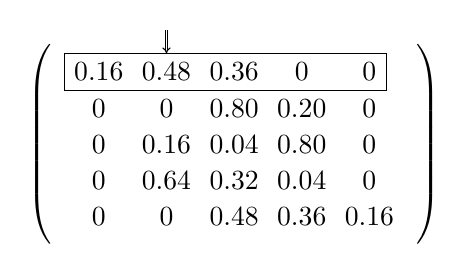
\begin{tikzpicture}
        \matrix [matrix of math nodes,left delimiter=(,right delimiter=)] (m)
        {
      	0.16 &0.48 &0.36 &0    &0\\
		0    &0    &0.80 &0.20 &0\\
		0    &0.16 &0.04 &0.80 &0\\
		0    &0.64 &0.32 &0.04 &0\\
		0    &0    &0.48 &0.36 &0.16\\
        };  
        \draw[color=black] (m-1-1.north west) -- (m-1-5.north east) --
        (m-1-5.south east) -- (m-1-1.south west) -- (m-1-1.north west);
        \draw[color=black,double,implies-](m-1-2.north) -- +(0,0.3);
    \end{tikzpicture}
\]



% %%%%%%%%%% %
% QUESTION 7 %
% %%%%%%%%%% %
\section*{Question 7}
An array of sojour times, or expect time spent in a nod before moving on :
\[E[R] = \left(\begin{array}{l}  1\\  2\\   4\\  
2.5\end{array}\right)\]
The array of computer return probabilitites for each state :
\[ p_{ii} = 1 - E[R]^{-1} = \left(\begin{array}{l}     0\\     1/2\\     3/4\\ 
3/5\end{array}\right) \] 
The reconstructed P matrix from the ebedded markov chain given :
\[P = \left(\begin{array}{llll}
  0 & 0.3(1) & 0.4(1) & 0.3(1) \\
0.1(1/2) & 1/2   & 0.2(1/2) & 0.7(1/2) \\ 
0.3(1/4) & 0.2(1/4) & 3/4   & 0.5(1/4) \\
0.4(2/5) & 0.4(2/5) & 0.2(2/5) & (3/5)
\end{array}\right)\]

% %%%%%%%%%%% %
% QUESTION 10 %
% %%%%%%%%%%% %

\section*{Question 10} 
\textbf{A.)} There are 6 states representing how many toys he has
\([S_0,S_1,S_2,S_3,S_4,S_5,S_6]\).
At each time step, he wil either recieve a new toy, moving to a higher state, or a
toy he already owns staying the same. as the number of toys he owns increasse
the probability of receiving a new toy decreases.
\\\[
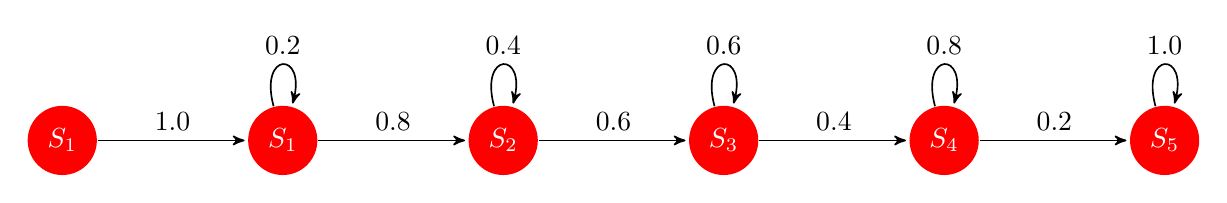
\begin{tikzpicture}[->,>=stealth',shorten >=1pt,auto,node distance=2.8cm, semithick] \tikzstyle{every state}=[fill=red,draw=none,text=white]

  \node[state]         (0)                    {$S_1$};
  \node[state]         (1) [right of=0]       {$S_1$};
  \node[state]         (2) [right of=1]       {$S_2$};
  \node[state]         (3) [right of=2]       {$S_3$};
  \node[state]         (4) [right of=3]       {$S_4$};
  \node[state]         (5) [right of=4]       {$S_5$};

  \path (0) edge              node {1.0} (1)
        (1) edge [loop above] node {0.2} (1)
            edge              node {0.8} (2)
        (2) edge [loop above] node {0.4} (2)
            edge              node {0.6} (3)
        (3) edge [loop above] node {0.6} (3)
            edge              node {0.4} (4)
        (4) edge [loop above] node {0.8} (4)
            edge              node {0.2} (5)
        (5) edge [loop above] node {1.0} (5); 
\end{tikzpicture}\]
\textbf{B.)} The transtion probability matrix :
\[P = \left(\begin{array}{llllll}
0&1  &0&0&0&0\\
0&1/5&4/5&0&0&0\\
0&0&2/5&3/5&0&0\\
0&0&0&3/5&2/5&0\\
0&0&0&0&4/5&1/5\\
0&0&0&0&0&1
\end{array}\right)\]
And the probability distribution of williams state after three happy meals :
\[
    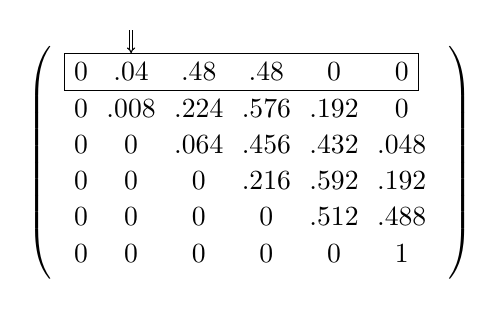
\begin{tikzpicture}
        \matrix [matrix of math nodes,left delimiter=(,right delimiter=)] (m)
        {
   0 &  .04 &  .48 & .48 &  0  & 0 \\
   0 &  .008 &  .224 &  .576 &  .192  & 0\\
   0 &  0 &  .064 &  .456 &  .432  & .048\\
   0 &  0 &  0 &  .216 &  .592  & .192\\
   0 &  0 &  0 &  0 &  .512  & .488\\
   0 &  0 &  0 &  0 &  0  & 1\\
        };  
        \draw[color=black] (m-1-1.north west) -- (m-1-6.north east) --
        (m-1-6.south east) -- (m-1-1.south west) -- (m-1-1.north west);
        \draw[color=black,double,implies-](m-1-2.north) -- +(0,0.3);
    \end{tikzpicture}
\]



\\\textbf{C.)} We want to discover $Se(S_0)$, that is, the mean time until
absorption for this Markov chain given we start in state 0, since we can see
that reaching $S_5$ is equivelent to reaching an absorbing state, and states
$S_0$ through $S_4$ are transient. 

\[ S = (I - T)^{-1} \]
\[T = \left(\begin{array}{rrrrr}
0&  1&  0&  0&  0\\
0&1/5&4/5&  0&  0\\
0&  0&2/5&3/5&  0\\
0&  0&  0&3/5&2/5\\
0&  0&  0&  0&4/5\\
\end{array}\right), \quad \quad S = \left(\begin{array}{rrrrr}
  1 & 1.25 &   1.66667 &  2.5  & 5 \\
  0 & 1.25 &  1.66667 &  2.5 &  5 \\
  0 & 0 &  1.66667  & 2.5 &  5 \\
  0 & 0 & 0 &  2.5 &  5\\
  0 & 0 & 0 & 0 &  5
\end{array}\right)\]
\[Var[S_e] = (2S - I)S_e - \mbox{sq}\{S_e\}\]
\[ Se = \left(\begin{array}{r}
   11.4167\\
   10.4167\\
    9.1667\\
    7.5000\\
    5.0000
\end{array}\right), \quad \quad Var[S_e] = 
\left(\begin{array}{r}
 25.174 \\
 25.174 \\
 24.861 \\
 23.750 \\
 20.000
\end{array}\right)\]

\\
\\The $E[T]$, the expected transtitions to absorbtions is 11.4167, and
the $Var[T]$, the variance is 25.174

\section*{Question 12}
Mean transition time was estimated using the following Octave function to
compute the M matrix
\begin{lstlisting}[frame=single] 
function j = mean_recurrence_time(P, n)
   if ( n == 1 ) 
       j = ones(size(P));
   else 
       M_1 = mean_recurrence_time(P, n-1);
       j = ones(size(P)) + P*(M_1 - M_1.*eye(size(M_1)) );
   endif
endfunction
\end{lstlisting}
Which was based off of the following relation 
\[ M^{(k+1)} = E + P(M^{(k)} - diag\{M^{(k)}), \mbox{with} M^{(0)} = E	\]
\\\(M^{256}\) was computed ( This was the limit before the recursive
implementation over flowed the function stack of Octave on my machine) At this
point its seems that the values had convereged sufficently to serve as a
reasonable approximation of the value as n approaches infinity. 
 \\\textbf{A.)} \(M_{22} \approx 2.3958\) 
 \\\textbf{B.)} \(M_{12} \approx 2.9167\)

\section*{Question 15}
Proof by Contradiction:
\\Assume states A and B are in the same communicating class,
that A is transient and that B is recurrent. 
\\
\\A being transient implies that if we are in state A, there is a non-zero
probability that you will never return to state A
\\
\\B being recurrent implies that if we are in state B, the probability to return
to B will alway be nonzero. 
\\
\\If B communicates with A then we must have a non-zero probability to travel
from B to A as well as a non zero probability to travel from A to B.
\\
\\Now assume that we start in state B and travel to state A, as must be possible
by the definition of communicating classes. Since A is transient there must be
some non-zero probability to never return to A. But since B is recurrent we will
always have a porbability to return to state B, and since B communicates with A
there is then a non zero probability to return to A. This means that there have
never me a non-zero probability to never return to A as there is always a
probability to return to A, a contradiction. 

  \section*{Question 17}
  \[P = \left( \begin{array}{rrrr}
  0.5 & 0.5 &   0 &   0 \\
  0.5 &   0 & 0.5 &   0 \\
  0.5 &   0 &   0 & 0.5 \\
    0 &   0 &   0 &   1
  \end{array}\right), \quad P^{(100)} =  \left( \begin{array}{rrrr}
  0 &   0 &   0 &   1 \\
  0 &   0 &   0 &   1 \\
  0 &   0 &   0 &   1 \\
  0 &   0 &   0 &   1
  \end{array}\right) \]
  Rasing the transition probability matrix to the hundreth power shows within
  resonable doubt that the states $[1,2,3]$ are transient, with state 4 being absorbing. 
  
  \[S = (I - T)^{-1}\]
  \[T=  \left( \begin{array}{rrr}
  0.5 & 0.5 &   0  \\
  0.5 &   0 & 0.5  \\
  0.5 &   0 &   0  \\
  \end{array}\right)\]
  \[S = \left( \begin{array}{rrr}
  8 & 4 & 2  \\
  6 & 4 & 2  \\
  4 & 2 & 2  \\
  \end{array}\right) \]
  
  \[R =\left( \begin{array}{rrrr}
  8 & 4 & 2 & \infty \\
  6 & 4 & 2 & \infty \\
  4 & 2 & 2 & \infty \\
  0 & 0 & 0 & \infty 
  \end{array}\right)\]
  \textbf{A.)}Expected number of visits to state 3, starting in state 1 : 2
  \\\textbf{B.)}Expected number of visits to state 1, starting in state 3 : 4
  \\\textbf{C.)}Expected number of visits to state 2, starting in state 4 : 0
  \section*{Question 20}
  In order to assist in the computation, I will add a state to represent the
  initail state 0. P' represent the new transtion probability matrix.
   \[ P' =\left(
  \begin{array}{rrrrrrrrr}
  0 & 0  & 0.4 & 0  & 0.6 & 0   & 0   & 0  & 0  \\
  0 & 0.6 & 0.4 & 0  & 0 & 0   & 0   & 0  & 0  \\
  0 & 0  & 0.2 & 0.6 & 0 & 0.2  & 0   & 0  & 0  \\
  0 & 0.2 & 0   & 0.3 & 0 & 0   & 0   & 0  & 0.5 \\
  0 & 0  & 0   & 0  & 0 & 0   & 0.9  & 0  & .1 \\
  0 & 0  & 0   & 0  & 0 & 0   & 1.0 &  0 & 0  \\
  0 & 0  & 0   & 0  & 0 & 0.5  & 0   & 0.5 & 0  \\
  0 & 0  & 0   & 0  & 0 & 1.0 & 0   & 0  & 0  \\
  0 & 0  & 0   & 0  & 0 & 0   & 0   & 0  & 1.0
  \end{array}\right)\]
  Examining the Marcov chain we can see that the states $[0,1,2,3,4]$ are
  transient, thus:
  \[S = (I - T)^{-1}\]
   \[ T' =\left(\begin{array}{rrrrr}
  0 & 0   & 0.4 & 0   & 0.6  \\
  0 & 0.6 & 0.4 & 0   & 0    \\
  0 & 0   & 0.2 & 0.6 & 0    \\
  0 & 0.2 & 0   & 0.3 & 0    \\
  0 & 0   & 0   & 0   & 0   
  \end{array}\right), \quad \quad S'= \left(\begin{array}{rrrrr}
   1 & .27 & .63 & .54 & .6 \\
   0 & 3.18 & 1.59 & 1.36 & 0 \\
   0 & .68 & 1.59 & 1.36 & 0 \\
   0 & .90 & .45 & 1.81 & 0 \\
   0 & 0 & 0 & 0 & 1
  \end{array}\right),\qaud \quad S'_e = \left(\begin{array}{r}
   3.05\\
   6.13\\
   3.63\\
   3.18\\
   1 \end{array}\right)\]
 \[Var[S'] = S(2*\mbox{diag}\{S\} - I) - \mbox{sq}\{S\}\] 
 \[Var[S_e] = (2S - I)S_e - \mbox{sq}\{S_e\}\]
   \[Var[S'] = \left(\begin{array}{rrrrr}
   0 & 1.38 & .98 & 1.14 & .24 \\
   0 & 6.94 & .94 & 1.73 & 0 \\ 
   0 & 3.19 & .94 & 1.73 & 0 \\
   0 & 4.04 & .78 & 1.48 & 0 \\
   0 & 0 & 0 & 0 & 0 
 \end{array}\right), \quad \quad Var[S'_e] = \left(\begin{array}{r}
    6.37\\
   15.50\\
   11.75\\ 
   12.72\\
    0 
  \end{array}\right)\]
  \textbf{A.)}Starting in state 0, the mean number of visits to state 1 is
  0.27273, varience is 1.38843 
 \\
 \\\textbf{B.)}Starting in state 0, the mean number of transitions
  before absorbtion is 3.0545, the varience is 6.37058
  
  
\section*{Question 23}
We compute the Absorbing chain from matrix P, to compute $\bar{P}$
\[
    \begin{tikzpicture}
        \matrix [matrix of math nodes,left delimiter=(,right delimiter=)] (m)
        {
  .6 & .4 & 0  & 0 & 0  & 0  & 0  & 0  \\
  0  & .2 & .6 & 0 & .2 & 0  & 0  & 0  \\
  .2 & 0  & .3 & 0 & 0  & 0  & 0  & .5 \\
  0  & 0  & 0  & 0 & 0  & .9 & 0  & .1 \\
  0  & 0  & 0  & 0 & 0  & 1  & 0  & 0  \\
  0  & 0  & 0  & 0 & .5 & 0  & .5 & 0  \\
  0  & 0  & 0  & 0 & 1  & 0  & 0  & 0  \\
  0  & 0  & 0  & 0 & 0  & 0  & 0  & 1  \\
        };  
        \draw[color=black] (m-1-5.north west) -- (m-8-5.south west);
        \draw[color=black] (m-1-8.north west) -- (m-8-8.south west);
        \draw[color=black] (m-8-1.north west) -- (m-8-8.north east);
        \draw[color=black] (m-5-1.north west) -- (m-5-8.north east)
    \end{tikzpicture}
\]
\[
    \begin{tikzpicture}
        \matrix [matrix of math nodes,left delimiter=(,right delimiter=)] (m)
        {
  .6 & .4 & 0  & 0 & 0  & 0   \\
  0  & .2 & .6 & 0 & .2 & 0  \\
  .2 & 0  & .3 & 0 & 0  & .5 \\
  0  & 0  & 0  & 0 & .9 & .1 \\
  0  & 0  & 0  & 0 & 1  & 0  \\
  0  & 0  & 0  & 0 & 0  & 1  \\
        };  
        \draw[color=black] (m-1-5.north west) -- (m-6-5.south west);
        \draw[color=black] (m-1-6.north west) -- (m-6-6.south west);
        \draw[color=black] (m-6-1.north west) -- (m-6-6.north east);
        \draw[color=black] (m-5-1.north west) -- (m-5-6.north east)
    \end{tikzpicture}
\]
We then compute S : 
 \[ T =\left(\begin{array}{rrrrr}
   0.6 & 0.4 & 0   & 0    \\
   0   & 0.2 & 0.6 & 0    \\
   0.2 & 0   & 0.3 & 0    \\
   0   & 0   & 0   & 0   
  \end{array}\right)\]
   \[ S =\left(\begin{array}{rrrrr}
     3.18  & 1.59 &  1.36 &  0.00\\
   0.68   &1.59 &  1.36  & 0.00\\
   0.91   &0.45 &  1.82  & 0.00\\
   0.00   &0.00 &  0.00  & 1.00 
     \end{array}\right)\]
Now we compute absorbtion probabilities, SB : 

   \[ B =\left(\begin{array}{rrrrr}
     0&0\\
   .2 & 0\\
   0 & .5\\
   .9 & .1 
     \end{array}\right)\]
     \[ SB =\left(\begin{array}{rrrrr} 
    0.318  & 0.682\\
   0.318  & 0.682\\
   0.091  & 0.909 \\
   0.900  & 0.100
          \end{array}\right)\]
\section*{Question 25}
\[P = =\left(\begin{array}{rrrrrr}
 q&p&0&0&0&\ldots\\
 q&0&p&0&0&\ldots\\
 0&q&0&p&0&\ldots\\
 0&0&q&0&p&\ldots\\
 0&0&0&q&0&\ldots\\
 \vdots&\vdots&\vdots&\vdots&\vdots&\ddots
\end{array}\right)\]
\textbf{A.)} The state machine would be ergodic if it has a z such that the sum
of z is 1, and zP = z. 

\[z_0 = qz_0 +pz_1 \longrightarrow z_0 - qz_0 = pz_1 \longrightarrow (1-q)z_0 =
pz_1 \longrightarrow pz_0 = pz_1 \]
\[\longrightarrow \underline{z_0 = z_1}\] 
\[z_1 = qz_0 + pz_2 \longrightarrow z_0 - qz_0 = pz_2  \longrightarrow (1-q)z_0 =
pz_2 \longrightarrow pz_0 = pz_2 \]
\[\longrightarrow \underline{z_0 = z_2}\] 
For all $k \in \mathbb{N},\quad z_n = z_{n-1}$ : 
\\\\\textbf{B.)}
\\Proof by induction.
\\Base case $z_2 = z_1$ is shown above since $z_0 = z_1 = z_2$.
\[z_n = qz_{n-1} + pz_{n+1}  \longrightarrow z_n = qz_n + pz_{n+1}
\longrightarrow z_n - qz_n = pz_{n+1} \longrightarrow (1 - q)z_n = pz_{n+1} \]
\[ \longrightarrow pz_n = pz_{n+1}  \longrightarrow \underline {z_n = z_{n+1}}\]

\section*{Question 26} This is a simple gamblers ruin problem. From the derivations from the notes, we
know the following equation holds : 
\[ x_i = \frac{1 - (p/q)^i}{1 - (p/q)^N}\]
From the problem, we know
\[ p = 18/38,\quad q = 20/38,\quad i = 10,\quad N=25.\]
Solving this equation gives 
\[x_{10} = \frac{1 - (\frac{18/38}{20/38})^{10}}{1 - (\frac{18/38}{20/38})^{25}}
\approx 0.701 \] 

\section*{Question 29}
\subsection*{\underline{$P_A$}}
\[P_A =\left(\begin{array}{rrr}
0.5&0.5&0\\
0&0.5&0.5\\
0.5&0&0.5
\end{array}\right)\]
\textbf{i.)}This has a stationart distribution, because the z vector
$(1/3,1/3,1/3)$ satisfies the requirement to be a stationary distribution. 
\newline
\textbf{ii.)} This has a limiting distribution, because 
\[\lim_{n\rightarrow\infty}{P_A^{n} }= \left(\begin{array}{rrr}
1/3&1/3&1.3\\
1/3&1/3&1/3\\
1/3&1/3&1/3
\end{array}\right)\]
and since this limit is defined it has a limiting distribution. 
\\\textbf{iii.)} Since the converging distribution is always $(1/3,1/3,1/3)$
regardless of initial state probabilities, there is a steady state dsitribution.

\subsection*{\underline{$P_B$}}
\[P_B =\left(\begin{array}{rrr} 0&1&0\\
0&0&1\\
1&0&0
\end{array}\right)\]
\textbf{i.)}This has a stationart distribution, because the z vector
$(1/3,1/3,1/3)$ satisfies the requirement to be a stationary distribution.
\newline
\textbf{ii.)} This does not have a limiting distribution since raising this
matrix to powers is periodic and itmwill never converge as n goes to infinity. 
\\\textbf{iii.)} Since this has no limiting distribution, it can have no steady
state distribution

\subsection*{\underline{$P_C$}}
\[P_C =\left(\begin{array}{rrrr}
.5&.5&0&0\\
.5&.5&0&0\\
0&0&.5&.5\\
0&0&.5&.5
\end{array}\right)\]
\textbf{i.)}This has a stationary distribution, because the z vector
$(1/4,1/4,1/4,1/4)$ satisfies the requirement to be a stationary distribution.
\\\textbf{ii.)}This has a limiting distribution since $P^n$ = $P^{n+1}$ and
raising this to the power of inifnity just equals P, therefore it converges.
\\\textbf{iii.)} Since the converging distribution depends on the initial state1
or 2, vs 3 or 4, there is not a steady state distribution. 

\subsection*{\underline{$P_D$}}
 \[P_D =\left(\begin{array}{rr} 1/n&(n-1)/n\\
(n-1)/n&1/n&
\end{array}\right)\]
\textbf{i.)}This has a stationary distribution, because the z vector
$(1/2,1.2	)$ satisfies the requirement to be a stationary distribution.
\\\textbf{ii.}
\[P_D^{k} = \frac{1}{2}\left(\begin{array}{rr}
\frac {1} {2} + \frac {1} {2} \left( \frac {2-n} {n} \right) ^ k &
\frac {1} {2} - \frac {1} {2} \left( \frac {2-n} {n} \right) ^ k \\
\frac {1} {2} - \frac {1} {2} \left( \frac {2-n} {n} \right) ^ k &
\frac {1} {2} + \frac {1} {2} \left( \frac {2-n} {n} \right) ^ k 
\end{array} \right)\]
As the figure $-n + 2 / n$ is less then 0 for all n, this figure approaches 0
as k goes to infinity, and thus :
\[\lim_{n\rightarrow\infty}{P_D^{n} = \left(\begin{array}{rrr}
1/2&1/2\\
1/2&1/2
\end{array}\right)\]
Therefore this has a limiting distribution.
\\\textbf{iii.)}Since the limit allways convergers to $(1/2, 1/2)$ regardless of
\end{array}
\end{document}
